%!TEX root = ../report.tex

\begin{document}
    \chapter{Theoretical Background}
    In this chapter the we will introduce the reader with the theoretical primers needed to comprehend this work in depth. 

    \section{Camera Geometry}
    A camera in simple words is mapping or projecting of 3d world points on an image plane. To understand how this mapping works we need to understand first the camera model which is defined using the tools of geometry. In computer there are two typed of camera models finite and infinite, which are divided on the basis of the distance of camera from the 3D real world points. In finite camera model the camera center lies at the finite distance distance from the 3D world point where this is vice versa in infinite camera model. In our case we will consider the finite camera model as it forms the basis of camera systems we use in the real world. 
    
    Generally the camera mapping or projection of 3d world point on the image plane is represented by camera matrix which is of size $3x4$, this matrix has 11 degrees of freedom. This matrix is can be divided into intrinsic and extrinsic camera matrix. To derive this camera mapping first we need to understand what is pin hole camera geometry. 
    
     \begin{figure}[h]
    \centering
    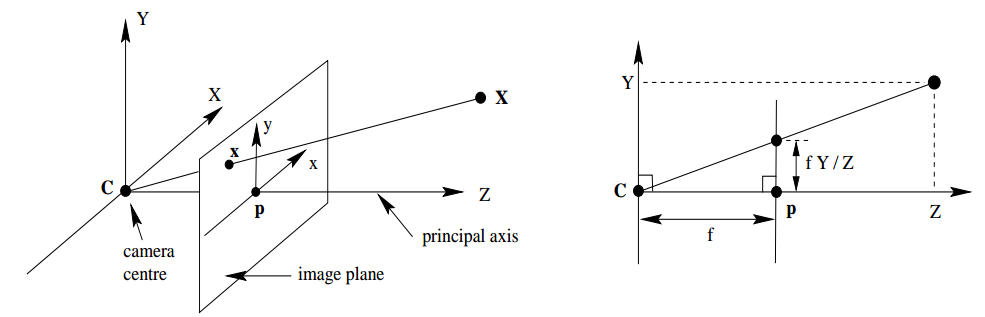
\includegraphics[width=\textwidth]{images/pinhole_camera.png}
    \caption{Pinhole camera geometry \cite{10.5555/861369}}
    \end{figure}
    
    Considering the central projection of 3D point \txtbf{X} on to the image plane. Let the camera center is at the center of origin of euclidean space. The image plane is at distance $z = f$. Pinhole camera model maps the point  \textbf{X} $ = (X, Y, Z)^{T}$ to the image plane, where a line from point \textbf{X} intersects the image plane at point \textbf{x} and meets the center of projection. This center of projection is also called camera center or optical center. Thus, using the similar triangles we can compute the mapping of $ (X, Y, Z)^{T}$ to $(fX/Z, fY/Z, f)^{T}$ which lies on the image plane. Therefore this projection can be seen as the mapping from $IR^{3}$ to $IR^{2}$ in euclidean space. 
    
    Assuming the world and image points to be homogeneous vectors this mapping can be represented as:
   \begin{center}
$\left(\begin{array}{c}X \\ Y \\ Z \\ 1 \end{array}\right) \rightarrow \left(\begin{array}{c} fX \\ fY \\ Z \end{array}\right) = \begin{bmatrix}f & & & 0 \\  &f & & 0  \\   & &1 & 0   \end{bmatrix}\left(\begin{array}{c}X\\ Y  \\Z \\ 1 \end{array}\right)$

\end{center}
    
The above equation can be represented as  $X^{‘} = PX $. Where X is the real world point represented in the homogenous coordinates as $(X, Y, Z, 1)^{T}$ and P is a $3x4$ homogeneous matrix called camera projection matrix. P in this case can be rewritten as $diag(f,f,1) [I|0]$, where diag(f,f,1) is a $3x3$ matrix and $[I|0]$ is a zero column vector. 
Generally the origin of coordinated is not at the optical center, there exists some offset. So the mapping in that case will change: 
\begin{center}
$(X,Y,Z)^{T} \rightarrow (fX/Z + p_{x}, fY/Z + p_{y})^{T}$
\end{center}
 where $(p_{x}, p_{y})^{T}$ are the coordinates of the new optical center. So according to this mapping can be expressed as:
   \begin{center}
$\left(\begin{array}{c}X \\ Y \\ Z \\ 1 \end{array}\right) \rightarrow \left(\begin{array}{c} fX + Zp_{x} \\ fY + Zp_{y} \\ Z \end{array}\right) = \begin{bmatrix}f & &p_{x} & 0 \\  &f &p_{y} & 0  \\   & &1 & 0   \end{bmatrix}\left(\begin{array}{c}X\\ Y  \\Z \\ 1 \end{array}\right)$

And $ K =  \begin{bmatrix}f & &p_{x} \\  &f &p_{y}  \\   & &1    \end{bmatrix}$
\end{center}
 Here K is called camera calibration matrix. The 3D world point is generally in the world coordinate frame and in most of the cases there exists some rotation and translation between the camera coordinate frame and world coordinate frame.
 
    \begin{figure}[h]
    \centering
    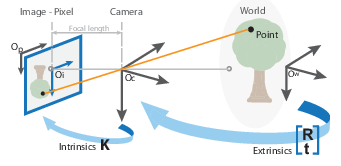
\includegraphics[width=8cm, height =4cm]{images/camera_geo.png}
    \caption{ Real world coordinates are transformed to camera coordinate frame using extrinsic matrix \cite{10.5555/861369}}
    \end{figure}
    
    This rotation and translation is generally represented as 3x4 matrix, $[R | C ]$ called extrinsic matrix, where $R$ is the rotation matrix and $C$ is the translation matrix. The above derived mapping assumes that the image plane is of similar scale in x and y direction, but in most of the cases it is not true. To counter this problem with the assumption that image coordinates are represented in the form of pixels we will introduce a scale factor here in x and y direction as $m_{x}$ and $m_{y}$ and we further introduce on more factor called skew coefficient $s$ in the cases when x and y axis of camera frames are not perpendicular to each other. Thus the resulting camera matrix can be represented as:
        \begin{center}
$K =  \begin{bmatrix} \alpha_{x} & s &c_{x} \\  0 & \alpha_{y} & c_{y}  \\  0  &0 &1 \end{bmatrix}$
    \end{center}
    
    So we can summarize this mapping from real world to camera plane, first the real world coordinates are transferred to camera coordinate frame via extrinsic matrix and the resulting points in camera coordinate frames are projected to image plane using camera matrix or instrinsic matrix. 
        \begin{figure}[h]
    \centering
    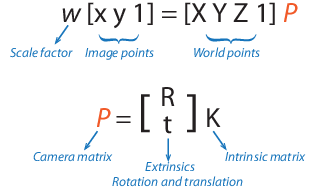
\includegraphics[width=8cm, height =4cm]{images/extrinsic_intrinsic.png}
    \caption{ Projection of a real world point onto image plane using camera geometry \cite{10.5555/861369}}
    \end{figure}
    
   
   
    \section{Inverse Perspective Mapping (IPM)}
     In computer vision inverse perspective transformation can be seen as a scenario where we obtain birds-eye-view image of the scene using front-facing camera image. To understand how the inverse perspective mapping we need to build some basic concepts about camera geometry which we discussed in the last section, homography and 2D perspective transformation. In autonomous driving IPM can be seen as an alternative way to feed the network with extra information about scene and it is explored in tasks like lane detection, BEV segmentation, path planning and more. 
     
     By definition homography is the way we can transform one projective plane to another plane using a transformation matrix called \textbf{H} and in this work we have used homography based IPM to take the front facing camera image to BEV. These transformation generally comes under the category of perspective transformation. Popularly there exists two types of transformations in projective geometry called as affine and perspective transformation. Example of affine transformation are translation, rotation, dilation. Affine transformations generally maps lines to lines, points to points and prallell lines stay parallel. Where as in the case of perspective transformation can hold only geometrical properties like will remain line and it retains col-linearity of points. Under perspective transformation two parallel lines can not stay parallel and they generally meet at a point at infinity which is called as vanishing point. The pin hole camera model that we have discussed above follows the principal of perspecitve transformation of a real world point to the camera image plane and the camera matrix that we have discussed is basically a homography matrix. Generally this camera matrix is obtained via association of 4 or more same points in the multiple images taken from same camera and this task is called camera calibration. 
     
            \begin{figure}[h]
    \centering
    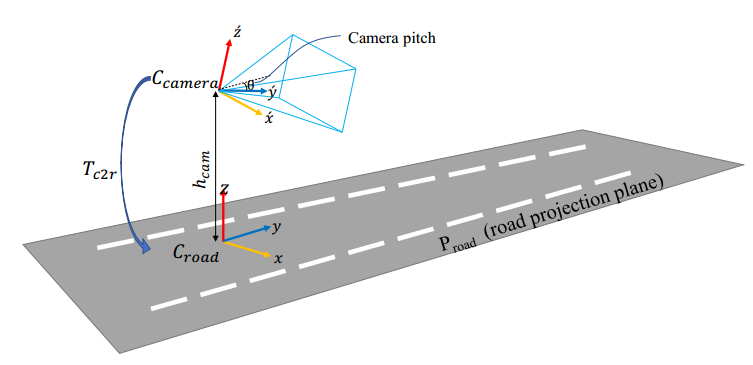
\includegraphics[width=8cm, height =4cm]{images/camera_geometry_lane_detection.png}
    \caption{ Geometric representation of a driving scenario \cite{DBLP:journals/corr/abs-1811-10203}}
    \end{figure}
    
     Most basic assumption in IPM is that we assume that the ground to be a flat plane and we then we map all the pixels from the front facing view to the flat ground plane with the help of homography. Moreover there exists some constraints for IPM to work like camera should be in fixed position as a small change in the position of camera can change the camera height and pitch with respect to the road and it can completely change how the scene is projected on the image plane, any object in the scene with certain height will cause distortions or artifacts in the BEV image and same can be seen with the points or objects lying above the ground. Now we will discuss in detail how to perform IPM. 
     
     \textbf{Step: A Define a top view region \newline} 
     First step for IPM is to define a top view region and we want this plane to be consistent with the moving vehicle. The origin of top view region plane is at the top left corner. Generally we start with deciding the width and height of this plane this defining the resolution per pixel. 
     
     Let $(ipm_{width}, ipm_{height} = 256, 416)$ and top view region edge points to be $[-10, 103], [10, 103], [-10, 3], [10, 3]$. Similary the IPM boundry points can be represented as $[0, 0],
                                                              [ipm_{width}, 0],
                                                              [0, ipm_{height}-1],
                                                              [ipm_{width}, ipm_{height}]$

     \textbf{Step: B Obtain homography from ipm to ground} \newline
     As mentioned above you need four or more points to calculate the homography matrix, via OpenCV you can obtain this by using cv2.getPerspectiveTransform\footnote{https://docs.opencv.org/3.4/da/d6e/tutorial_py_geometric_transformations.html} function. 
     Thus, obtaining $T^{ground}_{ipm}$
     
     \textbf{Step: C Obtain homography from ground to image} \newline
     Obtaining camera pitch, height and camera intrinsics and using camera projection matrix we can obtain the transformation from ground to image. 
     \begin{center}
     $T_{ground}^{camera } = \begin{bmatrix}1 & 0 & 0 & 0 \\0 & cos(\frac{\pi}{2} + pitch_{cam}) & -sin(\frac{\pi}{2} + pitch_{cam}) & height_{cam} \\ 0 &sin(\frac{\pi}{2} + pitch_{cam}) &cos(\frac{\pi}{2} + pitch_{cam}) & 0   \end{bmatrix}$
     \end{center}
     
     \begin{center}
     $T_{ground}^{image} = K . T_{ground}^{camera }$
    \end{center}
    
    
     \textbf{Step: D Obtain homography from image to ipm} \newline
    Until now we have $T^{image}_{ground}$ and $T^{ground}_{ipm}$
    
    \begin{center}
    $T^{image}_{ipm}$ = $T^{image}_{ground}$ X $T^{ground}_{ipm}$
    \end{center}
    
    \begin{center}
    $T^{ipm}_{image}$ = $(T^{ipm}_{image})^{-1}$
    \end{center}
    
    Using cv2.warpPerspective\footnote{https://docs.opencv.org/3.4/da/d6e/tutorial_py_geometric_transformations.html} again we can obtain our transformed image in BEV. 
    
    
\begin{figure}[h]
\centering
\begin{subfigure}{0.6\textwidth}
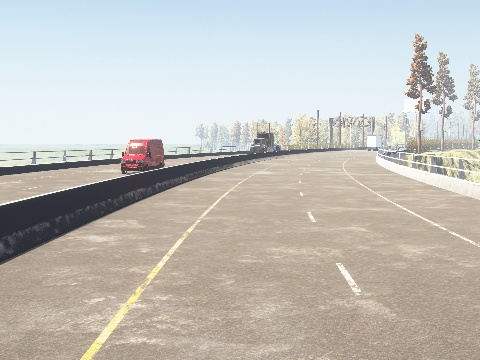
\includegraphics[width=1\linewidth, height=5cm]{images/report_image.jpg} 
\caption{}
\label{fig:subim1}
\end{subfigure}
\begin{subfigure}{0.4\textwidth}
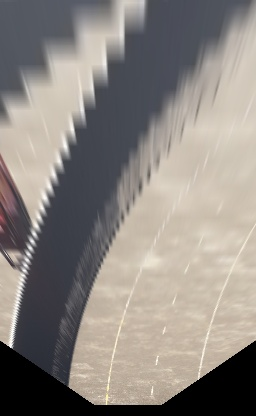
\includegraphics[width=0.5\linewidth, height=5cm]{images/report_image_ipm.jpg}
\caption{}
\label{fig:subim2}
\end{subfigure}

\caption{(a) Front facing camera driving scene taken from \cite{guo2020gen} and (b) BEV representation of the same driving scene}
\label{fig:image2}
\end{figure}
    
    \section{Hough Transform}
    
    The Hough transform is a feature extraction technique used in image analysis, computer vision, and digital image processing. The purpose of the technique is to find imperfect instances of objects within a certain class of shapes by a voting procedure. \footnote{https://en.wikipedia.org/wiki/Hough_transform}
    
    Generally Hough transform is used for detecting lines in an image but it is also applicable to detecting circles and ellipsoidal curves in an image. Hough transform is applied on images after edge detection is performed on it. Edge detection is a technique which identifies boundaries or edges of certain objects in the image on the basis of change in brightness across the pixels. Let's assume we are trying to find lines in an image, in that sense edges are sequence of pixels with certain slope and intercepts. To detect lines in this image we need to loop through all the pixels with same intercept and slope, this is where Hough transforms comes handy. In simple words Hough transform helps to find lines by giving weightage to the pixels that are already in a line. 
    
    Before indulging into the workings of the Hough transform, we need to understand the basic idea how the Hough transform works. A line can be represented by minimal two points and it has an intercept and a slope. Similarly a line can also be represented by a single point in mc space.
    
                \begin{figure}[h]
    \centering
    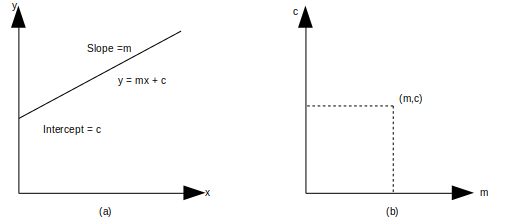
\includegraphics[width=10cm, height =4cm]{images/hough1.png}
    \caption{Representation of a line in (a) cartesian space (b) mc space}
    \end{figure}
    
    Similarly we can say that a point in cartesian space can be represented as infinite lines in mc space as infinite lines can pass from a point in cartesian space. So, Hough transform does the same converting points in cartesian space to lines in mc space. Therefore for an edge image, where the pixels are non black we can draw lines in mc space. Some lines will intersect at a particular point and that intersection point is this slope and intercept of those lines. 
    
                    \begin{figure}[h]
    \centering
    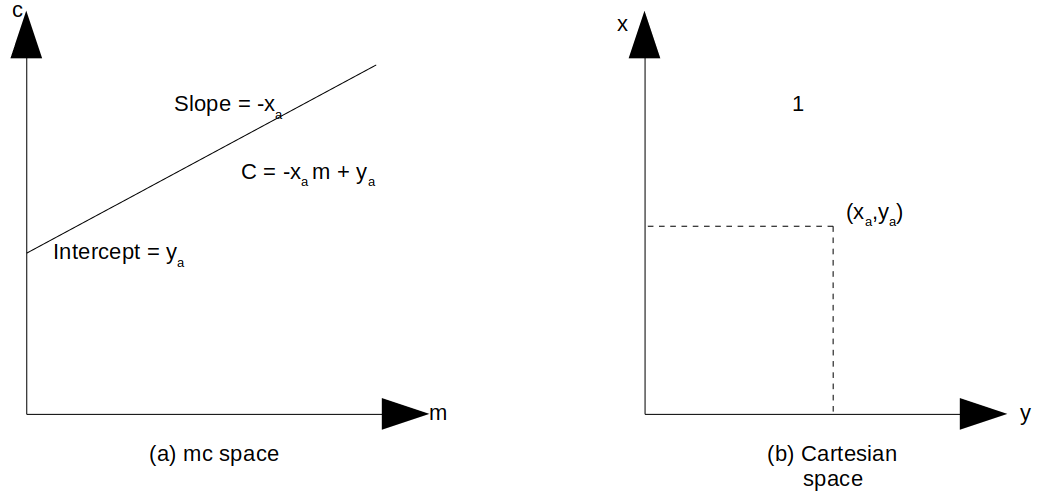
\includegraphics[width=10cm, height =4cm]{images/hough2.png}
    \caption{Representation of a point in (a) mc space (b) cartesian space}
    \end{figure}
    
    From the pixels points to line in mc space, when more than one lines intersects in mc space it means that those pixels belong to the same line in cartesian space and that line's parameter is represented by the intersecting point. 
    
                 \begin{figure}[h]
    \centering
    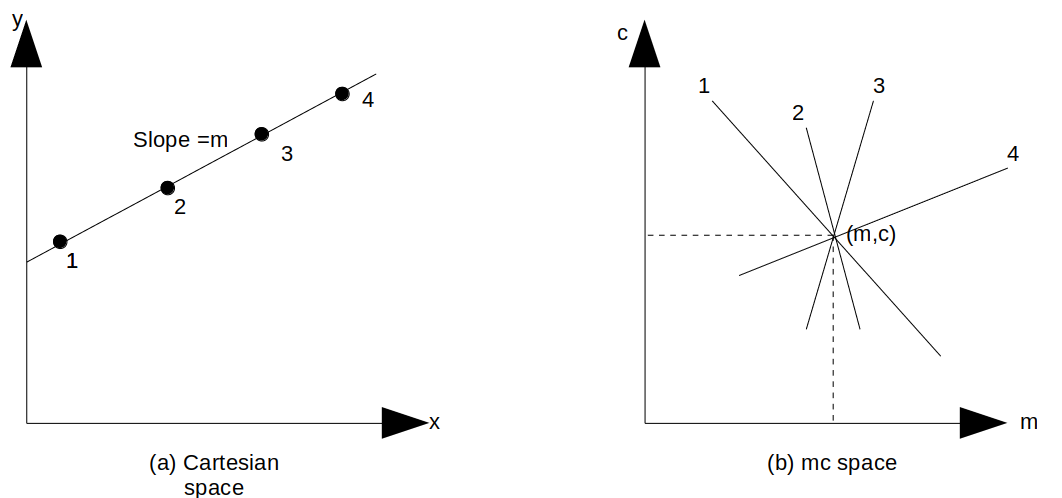
\includegraphics[width=10cm, height =4cm]{images/hough3.png}
    \caption{Representation of a point in (a) mc space (b) cartesian space}
    \end{figure}
    
    \section{A Brief Guide to Convolutional Neural Networks}
    
    \section{Semantic Segmentation}
    
\end{document}
